\section*{\SAPFEC{}}

\begin{frame}{General idea of \Pathfinding{}}

    \begin{block}{\Pathfinding{}}
        Given a weighted directed graph $\graph{o} = \paircs{\graphv{}}{\graphe{o}}$, $s, t \in \graphv{}$, \pathfinding{} is the task of computing a shortest-path from $s$ to $t$.
    \end{block}

    \begin{figure}
        \centering
        \begin{tikzpicture}
            \tikzset{Node/.style={circle, thick, draw=blue!80, fill=blue!40, minimum size=0.5cm}}
            \tikzset{OptimalPath/.style={circle, thick, draw=blue!80, fill=blue!40, minimum size=0.5cm}}

            \node[Node](N01) at (1,5) {$n_{1}$};
            \node[Node](N02) at (2,3.2) {$n_{2}$};
            \node[Node](N03) at (3,7) {$n_{3}$};
            \node[Node](N04) at (4,3) {$n_{4}$};
            \node[Node](N05) at (5,5.5) {$n_{5}$};
            \node[Node](N06) at (6,4) {$n_{6}$};
            \node[Node](N07) at (7,7) {$n_{7}$};
            \node[Node](N08) at (8,3) {$n_{8}$};
            \node[Node](N09) at (9,8) {$n_{9}$};
            \node[Node](N10) at (10,6) {$n_{10}$};

            \draw[-{Latex[length=2mm,width=3mm]}]
                (N01) edge node[above=1mm]{$7$} (N05) 
                (N01) edge node[above=1mm]{$1$} (N03) 
                (N03) edge node[above=1mm]{$7$} (N05)
                (N05) edge node[above=1mm]{$8$} (N10)
                (N04) edge node[left=1mm]{$5$} (N06)
                (N05) edge node[above=1mm]{$1$} (N07)
                (N07) edge node[above=1mm]{$1$} (N09)
                (N09) edge node[right=1mm]{$4$} (N10)
                (N06) edge node[below=1mm]{$4$} (N10)
            ;
            \draw[-{Latex[length=2mm,width=3mm]}, line width=0.8mm]
                (N01) edge node[right=1mm]{$2$} (N02) 
                (N02) edge node[above=1mm]{$3$} (N04)
                (N04) edge node[pos=0.2,above=2mm]{$2$} (N05)
                (N05) edge node[pos=0.2,right=2mm]{$2$} (N06)
                (N06) edge node[below=1mm]{$1$} (N08)
                (N08) edge node[below=1mm]{$2$} (N10)
                ;
        \end{tikzpicture}
    \end{figure}

\end{frame}

\begin{frame}{Compressed Path Database (\CPD{}) [Strasser 2014 et al.]}

    \vspace{-9pt}
    \begin{block}{}
        Given a graph, a \CPD{} is a data structure that efficiently stores the first edge of an optimal path from any node $s$ towards any node $t$.
    \end{block}

    \vspace{-2pt}
    \begin{minipage}{0.33\textwidth}
        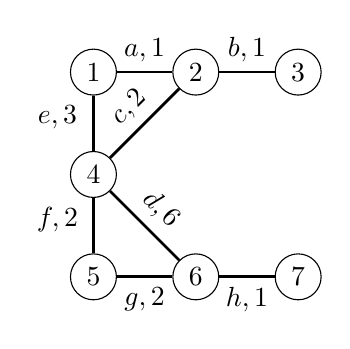
\begin{tikzpicture}
            \tikzset{Vertex/.style={%
                    shape=circle,%
                    draw=black,%
                    minimum size=10pt,%
                    radius=1cm,%
                    inner sep=3pt,%
                    node distance=1.3cm,%
                }}
        
                \node[Vertex] (1) {$1$};
                \node[Vertex, right of=1] (2) {$2$};
                \node[Vertex, right of=2] (3) {$3$};
                \node[Vertex, below of=1] (4) {$4$};
                \node[Vertex, below of=4] (5) {$5$};
                \node[Vertex, right of=5] (6) {$6$};
                \node[Vertex, right of=6] (7) {$7$};
        
                \path (1) edge[-,line width=1pt] node[above]{$a,1$} (2);
                \path (2) edge[-,line width=1pt] node[above]{$b,1$} (3);
                \path (4) edge[-,line width=1pt] node[above,sloped]{$c,2$} (2);
                \path (4) edge[-,line width=1pt] node[above,sloped]{$d,6$} (6);
                \path (4) edge[-,line width=1pt] node[above,xshift=-13pt,yshift=-6pt]{$e,3$} (1);
                \path (4) edge[-,line width=1pt] node[above,xshift=-13pt, yshift=-6pt]{$f,2$} (5);
                \path (5) edge[-,line width=1pt] node[below]{$g,2$} (6);
                \path (6) edge[-,line width=1pt] node[below]{$h,1$} (7);
        \end{tikzpicture}%
        \begin{center}%
            \vspace{-13pt}%
            $(s,t) = (2, 6)$%
        \end{center}
    \end{minipage}\hfill%
    \begin{minipage}{0.50\textwidth}
        \begin{center}
            \begin{minipage}{1.0\textwidth}
                \begin{minipage}{0.5\textwidth}
                    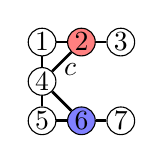
\begin{tikzpicture}
                        \tikzset{Vertex/.style={%
                                shape=circle,%
                                draw=black,%
                                minimum size=10pt,%
                                inner sep=0pt,%
                                node distance=0.5cm,%
                            }}
                    
                            \node[Vertex] (1) {$1$};
                            \node[Vertex, fill=red!50, right of=1] (2) {$2$};
                            \node[Vertex, right of=2] (3) {$3$};
                            \node[Vertex, below of=1] (4) {$4$};
                            \node[Vertex, below of=4] (5) {$5$};
                            \node[Vertex, fill=blue!50, right of=5] (6) {$6$};
                            \node[Vertex, right of=6] (7) {$7$};
                    
                            \path (1) edge[-,line width=1pt] (2);
                            \path (2) edge[-,line width=1pt] (3);
                            \path (4) edge[-,line width=1pt] node[xshift=3pt, yshift=3pt, below]{$c$} (2);
                            \path (4) edge[-,line width=1pt] (6);
                            \path (4) edge[-,line width=1pt] (1);
                            \path (4) edge[-,line width=1pt] (5);
                            \path (5) edge[-,line width=1pt] (6);
                            \path (6) edge[-,line width=1pt] (7);
                    \end{tikzpicture}
                \end{minipage}\hfill%
                \begin{minipage}{0.5\textwidth}
                    $CPD[2,6] = c$
                \end{minipage}

                \begin{minipage}{0.5\textwidth}
                    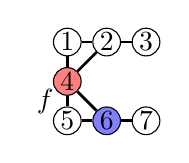
\begin{tikzpicture}
                        \tikzset{Vertex/.style={%
                                shape=circle,%
                                draw=black,%
                                minimum size=10pt,%
                                inner sep=0pt,%
                                node distance=0.5cm,%
                            }}
                    
                            \node[Vertex] (1) {$1$};
                            \node[Vertex, right of=1] (2) {$2$};
                            \node[Vertex, right of=2] (3) {$3$};
                            \node[Vertex, fill=red!50, below of=1] (4) {$4$};
                            \node[Vertex, below of=4] (5) {$5$};
                            \node[Vertex, fill=blue!50, right of=5] (6) {$6$};
                            \node[Vertex, right of=6] (7) {$7$};
                    
                            \path (1) edge[-,line width=1pt] (2);
                            \path (2) edge[-,line width=1pt] (3);
                            \path (4) edge[-,line width=1pt] (2);
                            \path (4) edge[-,line width=1pt] (6);
                            \path (4) edge[-,line width=1pt] (1);
                            \path (4) edge[-,line width=1pt] node[xshift=-8pt]{$f$} (5);
                            \path (5) edge[-,line width=1pt] (6);
                            \path (6) edge[-,line width=1pt] (7);
                    \end{tikzpicture}
                \end{minipage}\hfill%
                \begin{minipage}{0.5\textwidth}
                    $CPD[4,6] = f$
                \end{minipage}

                \begin{minipage}{0.5\textwidth}
                    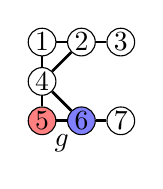
\begin{tikzpicture}
                        \tikzset{Vertex/.style={%
                                shape=circle,%
                                draw=black,%
                                minimum size=10pt,%
                                inner sep=0pt,%
                                node distance=0.5cm,%
                            }}
                    
                            \node[Vertex] (1) {$1$};
                            \node[Vertex, right of=1] (2) {$2$};
                            \node[Vertex, right of=2] (3) {$3$};
                            \node[Vertex, below of=1] (4) {$4$};
                            \node[Vertex, fill=red!50, below of=4] (5) {$5$};
                            \node[Vertex, fill=blue!50, right of=5] (6) {$6$};
                            \node[Vertex, right of=6] (7) {$7$};
                    
                            \path (1) edge[-,line width=1pt] (2);
                            \path (2) edge[-,line width=1pt] (3);
                            \path (4) edge[-,line width=1pt] (2);
                            \path (4) edge[-,line width=1pt] (6);
                            \path (4) edge[-,line width=1pt] (1);
                            \path (4) edge[-,line width=1pt] (5);
                            \path (5) edge[-,line width=1pt] node[yshift=-8pt]{$g$} (6);
                            \path (6) edge[-,line width=1pt] (7);
                    \end{tikzpicture}
                \end{minipage}\hfill%
                \begin{minipage}{0.5\textwidth}
                    $CPD[5,6] = g$
                \end{minipage}
            \end{minipage}

        \end{center}     
    \end{minipage}

    \vspace{-9pt}
    \begin{coloredBlock}{\CPDPathName{}}[OliveGreen][white]
        Given a graph $G$ and its \CPD{}, source node $s$ and target node $t$, 
        the $\CPDPath{s}{t}$ is the path obtained by concatenating edge $\CPD{}[s, t]$ with $\CPDPath{sink(\CPD{}[s, t])}{t}$ if $s \not = t$; the empty path otherwise.
    \end{coloredBlock}
\end{frame}

\begin{frame}{\A*{} [Nilsson et al., 1972]}
    \begin{block}{\A*{}}
        Given a (usually large) weighted directed graph representing a search space, an initial state $s$ and a set of goal states $T$, 
        the best-first search algorithm \A*{} computes a path from $s$ to a state in $T$.
    \end{block}

    \begin{itemize}
        \item node evaluation: $f(n) = g(n) + h(n)$;
        \item $g(n)$: cost of the path for reaching $n$ from $s$;
        \item $h(n)$: \textit{estimate} of the cost of the shortest-path for reaching a goal in $T$ from $n$;
        \item picks the best node $n$ found up until now, expands its successors and repeat until a goal is found.
    \end{itemize}

    \begin{block}{}
        If $h(n)$ is admissible (it never overestimate the actual cost of the shortest path from $n$ to a state in $T$), then \A*{} is optimal.
    \end{block}
\end{frame}